

\subsection{WP1: sequence similarity sketching}
In this package, the main objective is to design a randomized sketching that maps the sequences onto Euclidean space. 
The sketching function $\Phi\colon \abc^\star\to \RR^m$ is $(s_1,s_2, t_1,t_2)$-sensitive, if there exists similarity constants $0<s_1 < s_2<1$ and $t_1 < t_2$, and probabilities $c_1,c_2\in[0,1]$, such that for any two sequences $x,y\in\abc^\star$ it holds 
\begin{align}
\label{eq:sk_approx_factor}
\Prob{\ip{\Phi(x)}{\Phi(y)} > t_1 }\le c_1, && \text{if } \frac{\LCS(x,y)}{\max(|x|,|y|)}< s_1  \\
\Prob{\ip{\Phi(x)}{\Phi(y)} > t_2 }\ge c_2, && \text{if } \frac{\LCS(x,y)}{\max(|x|,|y|)}>s_2
\end{align}
where $\LCS(x,y)$ denotes the length of the longest common subsequence between $x$ and $y$, and the $\max(|x|,|y|)$ serves as the normalization factor.
While sketching $k$-mers by min-hashing has been studied extensively in the bioinformatics literature, de-Brujin sequences prove that $k$-mers cannot be used to derive bounds like equation~\eqref{eq:sk_approx_factor}. This motivates us to go beyond the local structures captured by $k$-mers and consider the global order of characters instead. Formally, for sequence $x\in \abc^\star$ and subsequence $a\in \abc^t$, define $T_x(a)$ as frequency sub-sequence $a$ in $x$ 
\begin{align}
 T_x(a):=\frac{1}{\binom{|x|}{t}}\# \set{(i_1,\dots,i_t)\in[|x|]^t: x_{i_1}\dots x_{i_t}=a, 1\le i_1<\dots<i_t\le |x|}.
\end{align}
It is evident that the size of $T_x(a)$ grows as $| \abc|^t$. In order to avoid the exponential dependency on $t$, we can lower the dimension of $T_x$ by random projections. Let $s_1,\dots, s_t\colon \abc\to \set{-1,1}$ be random sign functions and define sketch $\phi(T_x)=\sum_{a\in \abc^t} T_x(a)\prod_j^t s_j(a_j)$. Finally, let $\phi_1, \dots, \phi_m$ be $m$ independent copies of $\phi$, and define the sketching function as $\Phi(x):=1/\sqrt{m}(\phi_i(T_x))_{i\in[m]}$. 

Crucially, the sketching preserves inner product in expectation $\EE_\Phi \ip{\Phi(x)}{\Phi(y)} = \ip{T_x}{T_y}$ and the variance vanishes with more sketching dimensions $Var_\Phi \ip{\Phi(x)}{\Phi(y)}\propto 1/\sqrt{m}$, implying a space-accuracy trade-off. Furthermore, due to the low-rank design of the random hash functions, the sketching step $\Phi$ can be done implicitly, avoiding the exponentially large ambient space at all times. 

\paragraph{Deliverables}
\begin{itemize}
\item A publication describing the method for string edit distance sketching. 
\item An efficient implementation of the sketching method, plus experiments on some real-world genome datasets.
\end{itemize}


\subsection{WP 2: Phylogeny reconstruction}
The main focus of this work package is to develop a sub-quadratic sequence clustering algorithm based on our sketching scheme. Finding similar sequences is typically the most expensive step in phylogeny reconstruction. Therefore, ideas presented in this section can be exploited to reduce the complexity of phylogeny reconstruction, by avoiding the quadratic dependency on the number of sequences. 

Let $ \set{(x_i,g_i)}_{i\le N}$ be the list of $N$ sequences $x_i$, and their respective groups $g_i$. Furthermore, let us assume that similarity within each group is above $s_2$, i.e., $\LCS(x_i,x_j)\ge s_2, g_i=g_j$, while inter-group similarity is below $s_1$, i.e., $\LCS(x_i, x_j)\le s_1, g_i \neq g_j$, with $s_1 < s_2$ as constants. The task is to group sequences in an unsupervised fashion, which would be trivial by pairwise computation. However, we set out to avoid the quadratic dependency on $N$, by using discretized sketches. 

First, let $\phi_i(T_x)$s be tensor sketching functions as defined in work package 1, and define $\Phi'(x):=(\1 \set{\phi_i(T_x)}\ge 0)_{i\in [m]}$ to map the sketches onto binary hypercube $ \set{0,1}^m$. Furthermore, given sketches $h_i:=\Phi'(x_i)$, the bit-wise match probability between sketches $h_i$ and $h_j$ is equal to $\frac{1}{m}\ip{h_i}{h_j}$. Let $p_1$ ($p_2$) to the maximum (minimum) value of $\frac{1}{m}\ip{h_i}{h_j}$ for all pairs that belong to different groups $g_i\neq g_j$ (same group $g_i = g_j$):
\begin{align}
\label{eq:bit_match_prob}
% \begin{cases}
p_1=\max_{i\neq j} \set{\frac{1}{m}\ip{h_i}{h_j}\colon g_i \neq g_j},&&
p_2=\min_{i\neq j} \set {\frac{1}{m}\ip{h_i}{h_j} \colon g_i = g_j }.
% \end{cases}
\end{align}
By boosting the success probability, a sketch size $m:=\Ocal(\log(N))$ suffices for property \eqref{eq:sk_approx_factor} to hold for all $s_i,s_j$ simultaneously, ensuring that $p_1 < p_2$. 
Using random bit-sampling, we can amplify the ratio $\frac{p_1}{p_2}$. We construct $B$ blocks, $I_1,\dots,I_B$, each of size $b$. To construct $I_j=\{i_1,\dots, i_b\}$ select each bit \iid and \uar from the set of all bits: $i_1,\dots,i_b\sim\Unif[m]$. Let $h_{i|I_j}$ denote the $I_j$-induced sub-sketch $h_{i|I_j}:=h_i[i_1] h_i[i_2] \dots h_i[i_b]$. Using the bit-collision probabilities \eqref{eq:bit_match_prob}, we can calculate the block collision probabilities. 
For all $k\in[B],i,j\in[N]$, we have:
\begin{align}
&\Prob{\vee_{k=1}^B\ h_{i|I_k}= h_{j|I_k}}\le 1-(1-p_1^b)^B=:P_1 && g_i \neq g_j \\
&\Prob{\vee_{k=1}^B\ h_{i|I_k}= h_{j|I_k}}\ge 1-(1-p_2^b)^B=:P_2 && g_i = g_j 
\end{align}
With some calculation, it can be shown that for $B:=c N^\rho, b=\frac{\log(N)}{\log(1/p_1)}$, in which $\rho:=\frac{\log(1/p_2)}{\log(1/p_1)}$, we achieve $P_2\gtrsim 1-\E^{-c}$, and $P_1\lesssim c N^{-1+\rho}$ (for more details see~\cite{datar2004locality}). Based on these observations, if we iterate over all matching sketches we can find $1-e^{-c}$ of inner-group matches, while there are  $P_1\binom{N}{2} = \Ocal(N^{1+\rho})$ mismatches. Since we have $\rho<1$, the overall cost remains sub-quadratic $\Ocal(N^{1+\rho}\log(N))$. 





\paragraph{Deliverables}
\begin{itemize}
\item A publication detailing tensor sketching application for phylogeny reconstruction and its comparison to state of the art methods. 
\end{itemize}


\subsection{WP 3: Sketch-based alignment}
Based on the framework which we developed in the first two work packages, we can guide an alignment algorithm to achieve a better time-accuracy trade-off. Let us assume that the task is to find the nearest neighbors to a query sequence among reference sequences, ranked according to their edit distances. This nearest neighbor search can be viewed as an abstraction of read to genome alignment, with reference sequences representing $k$-mers of a genome, and query being a raw sequence read. Furthermore, the problem can be viewed as seed finding for seed and extend algorithms, with the query sequence representing substring of a second genome. 


Let $x \in \abc^\star, y\in \abc^\star$ be two sequences to be aligned. Let $\Lcal(x,y)$ denote the longest common subsequence $\Lcal(x,y):= \set{(i_1,j_1),\dots,(i_\ell,j_\ell)}$, where indices satisfy $x_{i_1}\dots x_{i_\ell} =y_{j_1}\dots y_{j_\ell}$, and $\ell:=\LCS(x,y)$ denotes the maximum possible length. Furthermore, indices must be strictly increasing $1\le i_1<\dots<i_\ell\le |x|$ and $1\le j_1<\dots<j_\ell\le |y|$. 

\subsubsection*{Guiding alignment}
Since computing optimal global alignment has a quadratic time complexity $\Ocal(|x||y|)$, it is considered inefficient if the query and references are millions of base-pairs long. However, one can reduce the time by restricting search space for alignment pairs. Some alignment tools break query and reference into $k$-mers, and use $k$-mer matches as seeds. Exact $k$-mer matching can be implemented efficiently using hash tables. However, the value of $k$ has to be sufficiently small to have a high chance of a match, and sufficiently big to avoid too many matches by chance. 
We propose sketch-matches as opposed to $k$-mer matches to be used as seed locations. Let $X_i:=x_i\dots x_{i+k-1}$ and $Y_i:=y_i\dots y_{i+k-1}$ denote $k$-mers of $x$ and $y$ respectively. Note that for most alignment pairs $(i,j)\in \Lcal(x,y)$, the corresponding $k$-mers $X_i,Y_j$ are likely to have a high degree of similarity $\LCS(X_i,Y_j)\ge s_2 k$, while for most of non-alignment pairs $(i,j)\notin \Lcal(x,y)$, the similarity must be lower $\LCS(X_i,Y_j)\le s_1 k$:
\begin{align}
 &(i,j)\sim \Lcal(x,y) \implies \Pr(\LCS(X_i,Y_j)\ge s_2 k) \ge c_1 \\
 &(i,j)\sim \overline{\Lcal(x,y)} \implies \Pr(\LCS(x,y)\ge s_1 k ) \le c_2,
\end{align}
where score thresholds $0< s_1 < s_2<1$ that depend on probabilities $0<c_1,c_2<1$ and value for $k$. 
Furthermore, we assume that sketching $\Phi: \abc^k\to\RR^m$ preserves the similarity order between $s_2$-similar $k$-mers $x,y\in \abc^k$ and $s_1$-dissimilar $k$-mers $x',y'\in \abc^k$, with constant probability
\begin{align}
 \LCS(x,y)\ge s_2 k,\LCS(x,y)\le s_1 k \implies \Pr\left(\|\Phi(x)-\Phi(y)\|_2\le \|\Phi(x')-\Phi(y')\|_2\right)\ge C,
\end{align}
where $0<C<1$ depends on constants $s_1,s_2$, as well as the accuracy of sketching function $\Phi$.
% In other words, the probability that an a random alignment pair will be closer than a random non-alignment pair after sketching will be at least $C$. 
If we restrict the search for alignment pairs to the neighbors of all $k$-mers $X_i$s and $Y_j$ based on distances $\|\Phi(X_i)-\Phi(Y_j)\|_2$, most alignment pairs will be found, while most non-alignment pairs will be excluded. The resulting candidate indices can be viewed as seed locations. 

The only quadratic term in the time complexity is $c_2 N^2$, corresponding to the pairs of indices that are similar $k$-mers but not part of the alignment. If we exclude highly self-similar sequences, we will have $c_2 = o(N)$, which would imply a sub-quadratic overall complexity.   



\paragraph{Deliverables}
\begin{itemize}
\item An implementation, as well as a publication, for read to reference alignment, using sensitive hashing values.
\end{itemize}


\subsection{WP 4: Syntenic region finding}
Syntenic regions are long ranges in assembled sequences that contain multiple closely related syntenic blocks. Moreover, these blocks may be inverted, translocated, or duplicated, due to evolutionary recombination or other factors. The goal of this work package is to devise a locality sensitive hashing scheme, to find and align these syntenic regions. However, before we can design such a scheme, we need to formally define a syntenic region. 


Let $x\in \abc^\star, y\in \abc^\star$ be two sequences, and let blocks refer to length $k$ substrings. For similarity thresholds $0\le s_1 < s_2\le 1$, any pair of blocks $X_i:=x[i:i+k-1]$ and $Y_j:=y[j:j+k-1]$ is either $s_2$-similar, $\LCS(X_i,Y_j)\ge s_2 k$, or $s_1$-dissimilar $\LCS(X_i,Y_j)\le s_1 k$. Syntenic blocks are defined as pairs of blocks $X_i$ and $Y_j$ that are $s_2$-similar. 

% Define bipartite graph $G$, with blocks $X_i$s and $Y_j$s as two disjoint sets, with an edge connecting the two if and only if $X_i$ and $Y_j$ form a syntenic block
% \begin{align}
% &G := (V_x\dot\cup V_y, E_{x,y}) \colon 
% \begin{cases}
% &V_x:=[|x|-k+1], \\
% &V_y:=[|y|-k+1]\\
% & E_{x,y}:= \set{(i,j)\in V_x\times V_y: \LCS(X_i, Y_j)\ge s_2 k}, 
% \end{cases} 
% \end{align}
% where $\dot\cup$ denotes disjoint union operation. 
% For blocks $i$ up to $i+\ell$ in $x$ and blocks $j$ up to $j+\ell$ in $y$, let $G'$ denote the subgraph of $G$ induced by these vertices. 
% \begin{align}
% &G':=\Big(V'_x\dot\cup V_y', E'_{x,y}\Big) \colon \begin{cases}
%  &V_x':=V_x\cap [i,i+\ell), \\
%  &V_y':=V_y\cap [j,j+\ell) \\
%  &E_{x,y}':= E_{x,y} \cap \big(V_x'\times V_y'\big)
%  \end{cases}
% \end{align}
%  The quadruple $(i,i+\ell, j, j+\ell)$ is a syntenic region if $G'$ has a matching that is $s'$-perfect, i.e., at least  $s' \ell$ edges will be part of the matching, where $s'\in[0,1]$ is a similarity constant. 
For $i,i'\in[|x|-k+1], j,j'\in[|y|-k+1]$ where $i\le i'$ and $j\le j'$, define syntenic region score, as the maximum number of syntenic blocks between $\set{X_i,\dots, X_{i'}}$ and $\set{Y_j,\dots, Y_{j'}}$
 \begin{align}
    \max_{\sigma\colon [i:i']\to[j:j']}\Big|\set{r\in [i:i']\colon \LCS(X_r,Y_{\sigma(r)})\ge s_2 k} \Big|
 \end{align}
where the maximization is taken over all injections from $\set{i,i+1,\dots, i'}$ to $\set{j,j+1,\dots, j'}$. 
\subsubsection*{Sketching the syntenic region score}
In this section, we focus on finding regions with fixed length $i'=i+\ell-1, j'=j+\ell-1$.  
We can employ the techniques outlined in the first package to match syntenic blocks. Subsequently, we can apply a second-level sketching. Therefore regions with a high percentage of syntenic blocks will remain close. Let $\Phi\colon \abc^k\to \set{0,1}^b$ be a $(s_1,s_2, p_1, p_2)$-sensitive sketching for blocks
\begin{align}
    &\LCS(X_i,Y_j)<s_1 k \implies \Prob{\phi_i(X_i)=\phi_i(Y_j)} < p_1, \\
    &\LCS(X_i,Y_j)>s_2 k \implies \Prob{\phi_i(X_i)=\phi_i(Y_j)} > p_2.
\end{align}
Let $\Xcal_i:=\Phi(X_i)$ and $\Ycal_j:=\Phi(Y_j)$ denote the set of sketches of blocks $X_i$ and $Y_j$, and define 
$\Scal_X:=\set{X_i,\dots,\Xcal_{i+\ell}}$ and $\Scal_Y:=\set{\Ycal_j, \dots, \Ycal_{j+\ell}}$ as the set of sketches within this region. 
% \begin{align}
%     &\Xcal_i:= \set{\Phi(X_i),\dots,\Phi(X_{i+\ell-1})},
%     &&\Ycal_j:= \set{\Phi(Y_i),\dots,\Phi(Y_{i+\ell-1})}.
% \end{align}
Let $\psi\colon (\set{0,1}^b)^\ell\to\set{0,1}^b$ be a min-hash sketch, using random permutation $\pi\colon\set{0,1}^b\to\set{0,1}^b$
\begin{align}
    &\psi(\set{h_1,\dots,h_\ell}):=\min_{i\in[\ell]} \pi(h_i)  && h_1,\dots, h_\ell\in \set{0,1}^b, \pi\colon \set{0,1}^b\to \set{0,1}^b.
\end{align}
The collision probability between $\psi(\Scal_X)$ and $\psi(\Scal_Y)$ is equal to $\frac{\alpha}{2-\alpha}$, where $\alpha$ is the normalized intersection $\alpha:=|\Scal_X\cap \Scal_Y|/\ell$. We can repeat this process $B$ times to improve sensitivity. 

It suffices to set $b:=\frac{\log(\ell)}{\log(1/p_1)}$ and $B:=c \ell^\rho$ for $\rho:=\frac{\log(1/p_2)}{\log(1/p_1)}$, to ensure that $1-e^{-c}$ of syntenic blocks are a match, while at most $c \ell^{1+\rho} $ non-syntenic blocks are matched. If we assume $p_1, p_2$ and $\rho < 1$ to be constants, determining if $(i,i+\ell, j, j+\ell)$ is a syntenic region requires $\ell^{1+\rho}$ time which remains sub-quadratic in the length of the region.  
% Finally, can retrieve matches between sketches by storing them in a hash table in $b B (|x|+|y|)\log(|x|+|y|)$ time, enabling us to retrieve syntenic regions with a high score in a quasi-linear time.




% \subsection{WP 4: Multi-scale graph backbone and visualization}
% Given a de-Brujin graph $G=(V,E)$, informally, we want a ``simple`` sequence graph $T$, such that for sequences in $G$, there is a corresponding sequence in $T$ that approximates it. While the primary goal of constructing $T$ is visualization, it can also represent major variations in the set, or clean a graph constructed from raw reads. Hypothetically, a concatenation of all the reference sequences as a long simple chain contains all reference sequences with no error, yet offers no further insight about the sequences. This motivates us to put some constraint on the size of $T$. We proceed by proposing a possible formalization:


% \subsubsection*{Minimum dominating set}
% Formally, $G=(V,E)$ is the de-Brujin graph and $v\in V$ are $k$-mers, and $w(v)$ denoting the multiplicity of this $k$-mer in all our reference sequences, and for vertices $u,v\in V$, $\D(u,v)$ denotes the shortest path distance on the graph. Moreover, $\mathcal{N}(v,k)$ denotes its $k$-step neighborhood of a vertex $\mathcal{N}(v,k):=\{u\in V\colon \D(u,v)\le k\}$, which can be extended to a subset of vertices $\mathcal{N}(S,k):=\cup_{v\in S}\mathcal{N}(v,k)(v,k)$ for $S\subseteq V$. We call such a subset $(C,k)$-dominating if $\sum_{v\notin \mathcal{N}(S,k)} w(v)\le C$, and let $\mathcal{D}(C,k)$ denote all $(C,k)$-dominating sets with minimum cardinality ($|S|$ is the least possible). 
% If $S\in \mathcal{D}(C,k)$, the sequence graph induced by $v(S)$ has $|S|k$ characters, and sum of the minimum distance of any $k$-mer in the reference sequences to $v(S)$ is bounded by $C$. 
% This optimization problem is NP-hard, as it contains a minimum dominating set problem as a special case. However, it admits approximation schemes that are efficient to compute. 

% \subsubsection*{Sketch-based visualization}
% The sketching scheme for syntenic region score can be readily used for visualization purposes. The first step is to visualize each genome sequence as separate paths, and if a syntenic region is found in multiple genomes, they will be joint at that location and diverge afterwards. On a lower abstraction level, the aligned syntenic blocks can be illustrated by bundling corresponding genomes, which then diverge at the location of syntenic breaks (gaps). One more detailed visualization would also indicate inverted blocks, as well as translocated and duplicated. 

% This technique can be generalized to a multi-level hierarchical scheme, with each sketch recursively computed based on the lower level sketches. The main idea is to build the de-Brujin graphs on multiple levels $k_\ell=k_0 K^\ell$, and use the sketches to collapse similar $k$-mers into a single vertex. $k_0$ is the smallest word size and $K$ determines how quickly the abstraction level grows. In order to avoid the redundancy between adjacent substrings, chosen $k_\ell$-mers are at least $k_\ell/c$-apart:
% $V_\ell:=  \set{s[i:k_\ell]\vert i\in \Ical_\ell}$, in which 
% $I_\ell:= \set{1,1+k_\ell/c,1+2k_\ell/c,\dots}$, and $k_0$ is divisible the absolute constant $c$. The edges at level $\ell$ are pairs of $k_\ell$-mers with a $k_\ell(1-1/c)$ overlap $E_\ell:= \set{(s[i:k_\ell],s[i+k_\ell/c:k_\ell]): i\in I_\ell}$. Moreover, let us assume that sketching functions $\Sk\colon \abc^{k_\ell}\to  \set{0,1}^m$ for all valid levels $\ell$, such that $\Sk(s[i:k_{\ell+1}])$ can be computed recursively using lower level sketches $\Sk(s[i:k_{\ell}])$. Furthermore, similarity edges $S_\ell$ are defined based on threshold $t$ for Hamming distance of sketches $S_\ell:= \set{(u,v)\colon \HD(\Sk(u),\Sk(v))/m\le t}$. 
% For the level $\ell$ de-Brujin graph $G_\ell:=(V_\ell,E_\ell)$, we construct backbone $T_\ell$ by copying $G_\ell$, and then contracting all similarity edges $S_\ell$ (contraction of edge $(u,v)$, removes $u$ and $v$ and creates $w$, and connects all incoming and outgoing edges to $w$). Since every $k_\ell$-mer can be uniquely mapped to a $k_{\ell+1}$-mer as its parent, vertices in $T_{\ell}$ can also be mapped to their parents in $T_{\ell+1}$. This hierarchical construction can be beneficial for characterization of genome differences, as well as multi-scale vizualization of multiple genomes. 


% In terms of organizational goals, visualizing syntenic blocks and regions, with the possibility to show multiple genomes at the same time, is the only concrete objective in this package. However, the hierarchical sketching and visualization are exploratory goals, and the objective may evolve during development and experiments. 


% More formally, for the reference sequence $s$, $V(k)$ denotes the set of $k$-mers $V(k):=  \set{s[i:k]\vert i\in \Ical_k}$, starting at indices $I(k):= \set{1,1+k/c,1+2k/c,\dots}$, in which $c$ is an absolute constant determining maximum overlap $k/c$. The edge set $E_k$ is comprised of adjacent $k$-mers $E(k):= \set{(s[i:k],s[i+k/c:k])\vert i\in I_k}$. Let $V(k_\ell),E(k_\ell)$ denote abstraction level $\ell$ vertices and edges for scale $k_\ell=C^\ell$, in which $C$ is an absolute constant. Moreover, let $\Sk(v)\in \set{0,1}^m$ denote a sketch function, that can be computed for all levels $v\in V(k_\ell)$, allows recursive computation of $\Sk(v)\in V(k_{\ell+1})$ based on $\Sk(v)\in V(k_\ell)$. Similarity edges $S(k_\ell)$ are defined using $t$ as similarity threshold $S(k_\ell):= \set{(u,v)\colon \HD(\Sk(u),\Sk(v))/m\le t}$. Finally, if $G_\ell=(V(k_\ell),E(k_\ell))$ denotes the de-Brujin graph at level $\ell$, and backbone graph $T_\ell$ is defined by contraction of all similarity edges on $G_\ell$ (contraction of edge $(u,v)$, removes $u$ and $v$ and creates $w$, and redirects all incoming and outgoing edges towards $w$).


% For example, let $h_i:=\Sk(s[5i+1:10]), h_i\in \set{0,1}^m$ denote the sketches for $10$-mers of the reference sequence $s$. Consequently, the sketch for $s[1:100]$ is recursively computed on sequence $h_0[I],\dots,h_{19}[I]$, and repeated with \iid subsampled index set $I\subseteq[m]$. The desired number of scales for visualization can be tuned by choosing the cardinality of sub-index set $|I|$, recursion factor, and overlap factor.~\footnote{recursion factor $C$ means $k$-mer sketches are computed based on $k/C$-mer sketches. Overlap factor $C$ means only for $k$-mers at indices $1,1+\floor{k/C},1+\floor{2k/C},\dots$ the sketches are computed.}.
% \subsubsection*{Random walk, leverage scores }
% Similar to before, let $V$ denote the set of all $k$-mers in our dataset. However, for any two 
% The sketching scheme outlined to find syntenic regions, can be used to add extra edges to sequence graph, indicating 
% In the same setting for $G$, plus a root node $r\in V$ that can reach all other nodes, we compute random spanning trees: starting from $r$ take out-going edges at random, in a breadth-first fashion to construct tree $T_1$, and repeat this $\ell$ times. For each node $v$, let the score $s_i(v)$ corresponding to $T_i$ is defined the number of its descendants, the overall score is defined as the sum $s(v):=\sum_i s_i(v)$. Finally, we find the subset $S\subseteq V$, such that $G[S]$ is connected and $\sum_{v\in S} w(v)s(v)$ is maximized. The rationale behind this is that, $s(v)$ is correlated with the length of a random-walk initiated at $v$. 







\paragraph{Deliverables}
\begin{itemize}
% \item A visualization algorithm and a publication, for visualization of multiple reference genomes on different abstraction scale.
% \end{itemize}
% \paragraph{Deliverables}
% \begin{itemize}
\item A manuscript and an implementation of this approach, with application on simulated data, and two whole-genome references that are not very closely related. 
\end{itemize}

% \subsection{Sketch-based optimization}









% %% Your work plan should be presented in terms of work packages, each work package representing a major piece of work. The number and nature of the work packages will depend on the topic of research and this is where the student should be guided by their supervisor. As a general guideline, a work package should describe a minimum of 3 and a maximum of 12 months of work. Each work package description should define the task and the expected outcomes. 

% %% \subsection{WP 1: My First Work Package}
% %% \paragraph{First Part of WP 1}
% %% Text goes here... lots of text.

% %% \begin{figure}[ht]
% %% \centering
% %% 	\subfloat[]{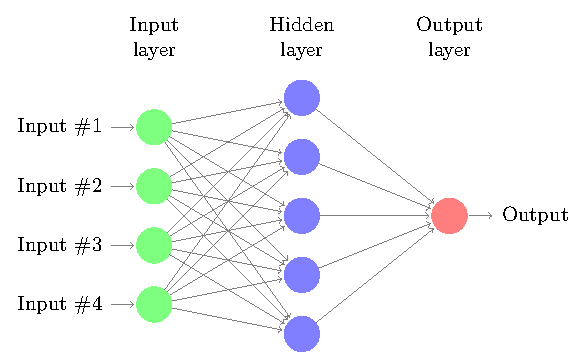
\includegraphics[width=.49\linewidth]{figures/neural-network.pdf}\label{fig:nnA}} \hfill
% %% 	\subfloat[]{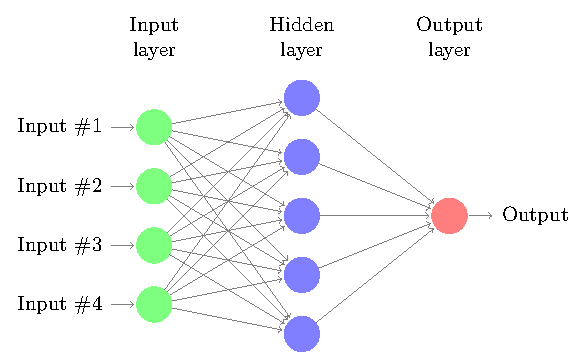
\includegraphics[width=.49\linewidth]{figures/neural-network.pdf}\label{fig:nnB}} \\
% %% \caption{\textbf{A.} A neural network. \textbf{B.} The same neural network.}
% %% \label{fig:universes}
% %% \end{figure}

% %% \subsection{WP N: Writing the Dissertation}
% %% Writing the dissertation is planned. Things never go as planned.

% The proposed research mainly focuses on machine learning algorithms addressing the four main challenges in clinical data: heterogeneous sampling rate, irregular sampling rate, missing variables and different modalities of data.
% In the end these algorithms will be integrated into one framework which is the final goal of the proposal.
% The framework will be evaluated and compared with each algorithm alone to check if combining them will lead to improvement in performance.
% The following work packages present the outline of the main phases to tackle the research questions.

% \subsection{WP 1: Early-warning system for organ deterioration}
% In this workpackage we use ICU data collected from the ICUs of University Hospital Bern, which will be referred as Bern ICU data.
% The raw Bern ICU data come directly from the patient data management system (PDMS) of the hospital, which contains lots of artifacts caused by people misentering dates, values or variable IDs of the records.
% There are sometimes multiple records with different of the same variable for the same patients at the same time, which causes confusion because we do not know which one contains the correct measurement value.
% These artifacts need to be cleaned out before we use the data to train early-warning models.

% There exists more than 5000 variables in the Bern ICU data but not all are relevant to the organ deterioration tasks of interest, and also some are only used for short term like in clinical trails which lead to high sparseness.
% We only select variables that are most relevant to the prediction tasks as well as measured for most of the patients over most of the years in the dataset to reduce the sparseness in the final set of data that is used to train the early-warning system.
% The variable selection will be done by analyzing the statistics of the variables and with the professional knowledge from clinicians.

% After artifact cleaning and feature selection, we need to transform the data from tables to feature matrices that machine learning models can use as inputs.
% A patient will be represented by a matrix where each row corresponds to a time step and each column corresponds to a variable.
% In such matrices, there are many entries with missing values due to the heterogeneous and irregular sampling rate as well as the missing variables, which will be manually imputed.
% Labels of future organ deterioration will be computed from non-imputed data based on the definition provided by the clinicians. 
% Both non-sequential models, such as logistic regression or lightGBM, and sequential models like LSTMs will be used to predict organ deteriorations within the next 8 hours, the best one among which will be selected.
% This workpackage, where missing variables are imputed manually, establishes a baseline for the future work packages where deep learning models that can directly take non-imputed data as inputs. 

% This work is done in collaboration with Stephanie Hyland, Matthias H\"{u}ser, Martin Faltys and Tobias Merz.

% %% For the purpose of training and evaluation of the proposed algorithms and the final framework, clinical data are needed.
% %% One available clinical dataset is the ICU data collected from our collaborator, ``the University Hospital of Bern.
% %% Besides the Bern ICU dataset, two open-access ICU datasets will also be used: the MIMIC-III dataset \cite{saeed2011multiparameter} and the Philips eICU dataset \cite{mcshea2010eicu}.
% %% Since all the datasets used in the proposed research are collected from ICU, the data sampling rate usually ranges from every few minutes to once a few days.
% %% Table \ref{tbl:data} summarizes some basic information of these three datasets.
% %% \begin{table}[!ht]
% %% \caption{Summary of the three ICU datasets we will use in the proposal.}
% %% {\footnotesize
% %% \begin{tabular}{p{0.225\textwidth} p{0.225\textwidth} p{0.225\textwidth} p{0.225\textwidth}}
% %% \midrule
% %% ~ & \textbf{MIMIC-III} & \textbf{Phillips eICU} & \textbf{University Hospital Bern} \\ \midrule
% %% \textbf{No. of patients} & 46,520 & 139,367 & 55,476 \\ \midrule
% %% \textbf{No. of variables} & 13,240 & 2,905 & 5,178 \\ \midrule
% %% \textbf{No. of measurements} & $\approx 312\times10^6$ & $\approx 827\times10^6$ & $\approx 3,469\times10^6$ \\ \midrule
% %% \textbf{Highest resolution} & $\approx 15$ minutes & $\approx 5$ minutes & $\approx 2$ minutes \\ \midrule
% %% \textbf{Time range} & 2001 to 2012 & 2014 to 2015 & since 2005 \\ \midrule
% %% \textbf{Demographics} & Patients at Beth Israel Deaconess Medical Centre (Boston, USA) & Patients from 459 critical care units across continental USA & Patients at University Hospital Bern (Switzerland) \\ \midrule
% %% \end{tabular}}
% %% \label{tbl:data}
% %% \end{table}

% %% While acquiring access to these ICU datasets is not difficult, the data do not come in a format that can be directly used by the proposed algorithms, so preprocessing the data into the desired format is an important task in this phase.
% %% Another problem is that the number of clinical variables is very large, however, a large amount of them were rarely observed.
% %% These rare variables may be observed only in some very specific patients or used in some short-term clinical trials, therefore not suitable for the general clinical problems.
% %% So one other important task in this phase is extracting commonly used and clinically important variables for general purposes.

% %% The raw ICU data directly from the patient data manangement system (PDMS) usually contain many artifacts caused by people misentering dates, values or variable ID of the observsations, or sometimes entering the same records multiple times and etc.
% %% While there are fewer artifacts in the MIMIC-III dataset and the eICU dataset because they might have been cleaned before people publish them, the Bern ICU dataset still contains quite some amount of artifacts that could significantly degrade the model peformance if ignored.
% %% Therefore, one additional task for the Bern ICU dataset is data cleaning.

% \paragraph{Deliverables}
% \begin{itemize}
% \item A set of programs that clean up the Bern ICU data, preprocess tables of ICU records and transform them into feature matrices.
% \item A medical journal paper on ICU Bern organ deterioration early-warning system.
% \end{itemize}

% \subsection{WP 2: Unsupervised representation learning from single data modality}
% This workpackage uses data from the Philips eICU dataset \cite{mcshea2010eicu}, which consists of 139367 patients and 2905 variables collected from 459 different critical care units across continental USA.
% Artifacts cleaning, feature selection, data format transformation and manual imputation also need to be applied, same as the preprocessing steps in WP 1.
% We compare non-sequential and sequential unsupervised learning techniques in terms of the representation performance in both reconstruction and prediction.
% In order to have a more objective evaluation on the generality of patients representations, we need to design a list of clinically related prediction tasks that covers a wide range of clinical concepts.
% The dynamic diagnosis and treatment records satisfy such requirement. 

% The non-sequential unsupervised representation learning techniques we use are PCA and vanilla autoencoder, and the sequential ones are variations of sequence-to-sequence model.
% Sequence-to-sequence models can be used as an autoencoder, i.e. the decoder reconstructs the input sequences; but it can also be used as a forecaster, which predict the future sequence of the current input sequences.
% Between a forecaster and an autoencoder with the same number of parameters, a forecaster has the advantage of ``seeing'' some future information than just the history during training, hence representations learned by the forecasters should be more predictive of the future events.
% Attention mechanism will also be added to the sequence-to-sequence forecaster under the intuition that feature values at each future time point may have higher relevance to only a local region of the input sequence. 

% \paragraph{Deliverables}
% \begin{itemize}
% \item A conference paper that benchmarks the unsupervised representation learning methods on medical time series.
% \end{itemize}

% \subsection{WP 3: Learning from multirate irregular time series}
% The data used for this workpackage are the commonly observed numerical variables.
% Missing variables will be imputed with global mean or expert-defined normal values.
% The data will be resampled to be on a fixed-interval time grid to remove the irregularity.
% Sampling rate of the data will be made sure to be in these three range: every few minutes, every few hours and once a day.
% In the baseline method, the time series will be imputed with forward-filling.

% The clinical problem of interest is learning representations that can be used to predict diagnosis/treatments in the future. 
% Different representation learning methods in a either supervised or unsupervised fashion will be studied in order to establish the best baseline.
% In the best representation learning model, the parts that takes the time series as inputs will be replaced with Phased LSTM, multi-rate LSTM and the proposed algorithm respectively, so that it will be able to take non-imputed multi-rate time series as inputs, and the former two will be the state-of-the-art baseline for the last one to compare against.
% The performance of the proposed method and the baselines will be evaluated on the representation performance in the diagnosis/treatment prediction tasks.

% Two naive baselines will be used in dealing with irregularity, in both of which standard LSTMs will be used, but one will ignore the irregularity by ``pretending'' that two consecutive observations always have a fixed time interval and the other uses data resampled to a fixed-interval time grid.
% Besides the two naive baselines, the proposed method will also be compared with T-LSTMs as the state-of-the-art baseline.
% \paragraph{Deliverables}
% \begin{itemize}
% \item Design, definition and implementation of the proposed algorithm.
% \item Two conference papers will be written presenting the proposed algorithms.
% \end{itemize}

% \subsection{WP 4: Learning from time series with missing variables}
% The data used in this work package will still be similar to those in WP 2, with the only difference that the missing variables will not be imputed.
% Since the research at this phase focuses on dealing with missing variables, the time-series will also be forward-imputed to remove the multirate aspect.
% The clinical problem is diagnosis prediction or medicine recommendation.

% Standard LSTMs will be applied to the data with missing variable values imputed by the statistical global mean or the expert-defined normal values.
% Methods and metrics to measure the similarity between time series will be designed so the temporal components can also be incorporated into the CF framework for the clinical problem.
% \paragraph{Deliverables}
% \begin{itemize}
% \item Design of the similarity measurement method and metric for time series.
% \item A conference paper will be written presenting CF over clinical time series with missing variables.
% \end{itemize}

% \subsection{WP 5: Representation learning from heterogeneous data modalities}
% In this work package, we will implement a joint model that combines Med2Vec \cite{choi2016multi} and the representation learning algorithm for numerical clinical variables developed in WP 2.
% Representations learned from the joint model will be compared with the Med2Vec representations and WP-2 representations in terms of their prediction performance in the organ deterioration early-warning task mentioned in WP 1. 

% %% In this work package, the methods from WP 2, 3, 4 will be integrated into a united model that uses only numerical time-series data as input.
% %% Time series of texts will be encoded into time series of word embeddings using GloVe, and time series of medical codes will be encoded by Med2Vec.
% %% The time series of embeddings will be treated the same as the numerical time series and be input to the aforementioned combined time-series model.
% %% The entire framework will be compared with the combined model that only uses numerical clinical variables to check if incorporating more data will improve the performance.
% \paragraph{Deliverables}
% \begin{itemize}
% \item A represenation model that take both numerical clinical variables and medical codes as inputs.
% \end{itemize}

% \subsection{WP 6: Writing the Dissertation}
% Writing dissertation to summarize all the previous works.
